% ============================================================================
% CHAPTER 3: SYSTEM DESIGN
% ============================================================================

\chapter{SYSTEM DESIGN}

\section{SYSTEM ARCHITECTURE}

This section presents the detailed architecture of the EEG-based depression detection system, describing the complete processing pipeline from raw signal acquisition through classification and explainability analysis. The architecture reflects a careful balance between model expressiveness, computational efficiency, and interpretability requirements.

\subsection{Complete Pipeline Overview}

The system processes raw EEG signals through a multi-stage pipeline that transforms continuous recordings into depression classification predictions accompanied by comprehensive explainability outputs. The pipeline begins with data loading, where EDF-format recordings are parsed to extract the 19-channel EEG signals. These raw signals undergo extensive preprocessing including filtering, artifact removal, and epoch segmentation to produce clean, standardized input suitable for feature extraction.

The feature extraction stage branches into two parallel pathways. The first pathway computes Wavelet Packet Decomposition features that capture fine-grained spectral information across 32 frequency subbands, yielding 576 features per channel that serve as node attributes for the Graph Attention Network. The second pathway generates Continuous Wavelet Transform scalograms that represent the time-frequency evolution of the signal in a 64×128 image format suitable for the Vision Transformer. These parallel feature representations feed into their respective model branches, which process the information through specialized architectures optimized for their input modalities.

The Transformer and GNN branches produce fixed-dimensional feature vectors that are combined through an attention-based fusion module. This fusion mechanism learns to adaptively weight the contributions from each branch based on the characteristics of the input, producing a unified representation that captures both time-frequency patterns and spatial electrode relationships. The fused features pass through a classification head that outputs a depression probability, and the complete forward pass supports gradient-based explainability methods that reveal which input features drove the prediction.

\begin{figure}[H]
    \centering
    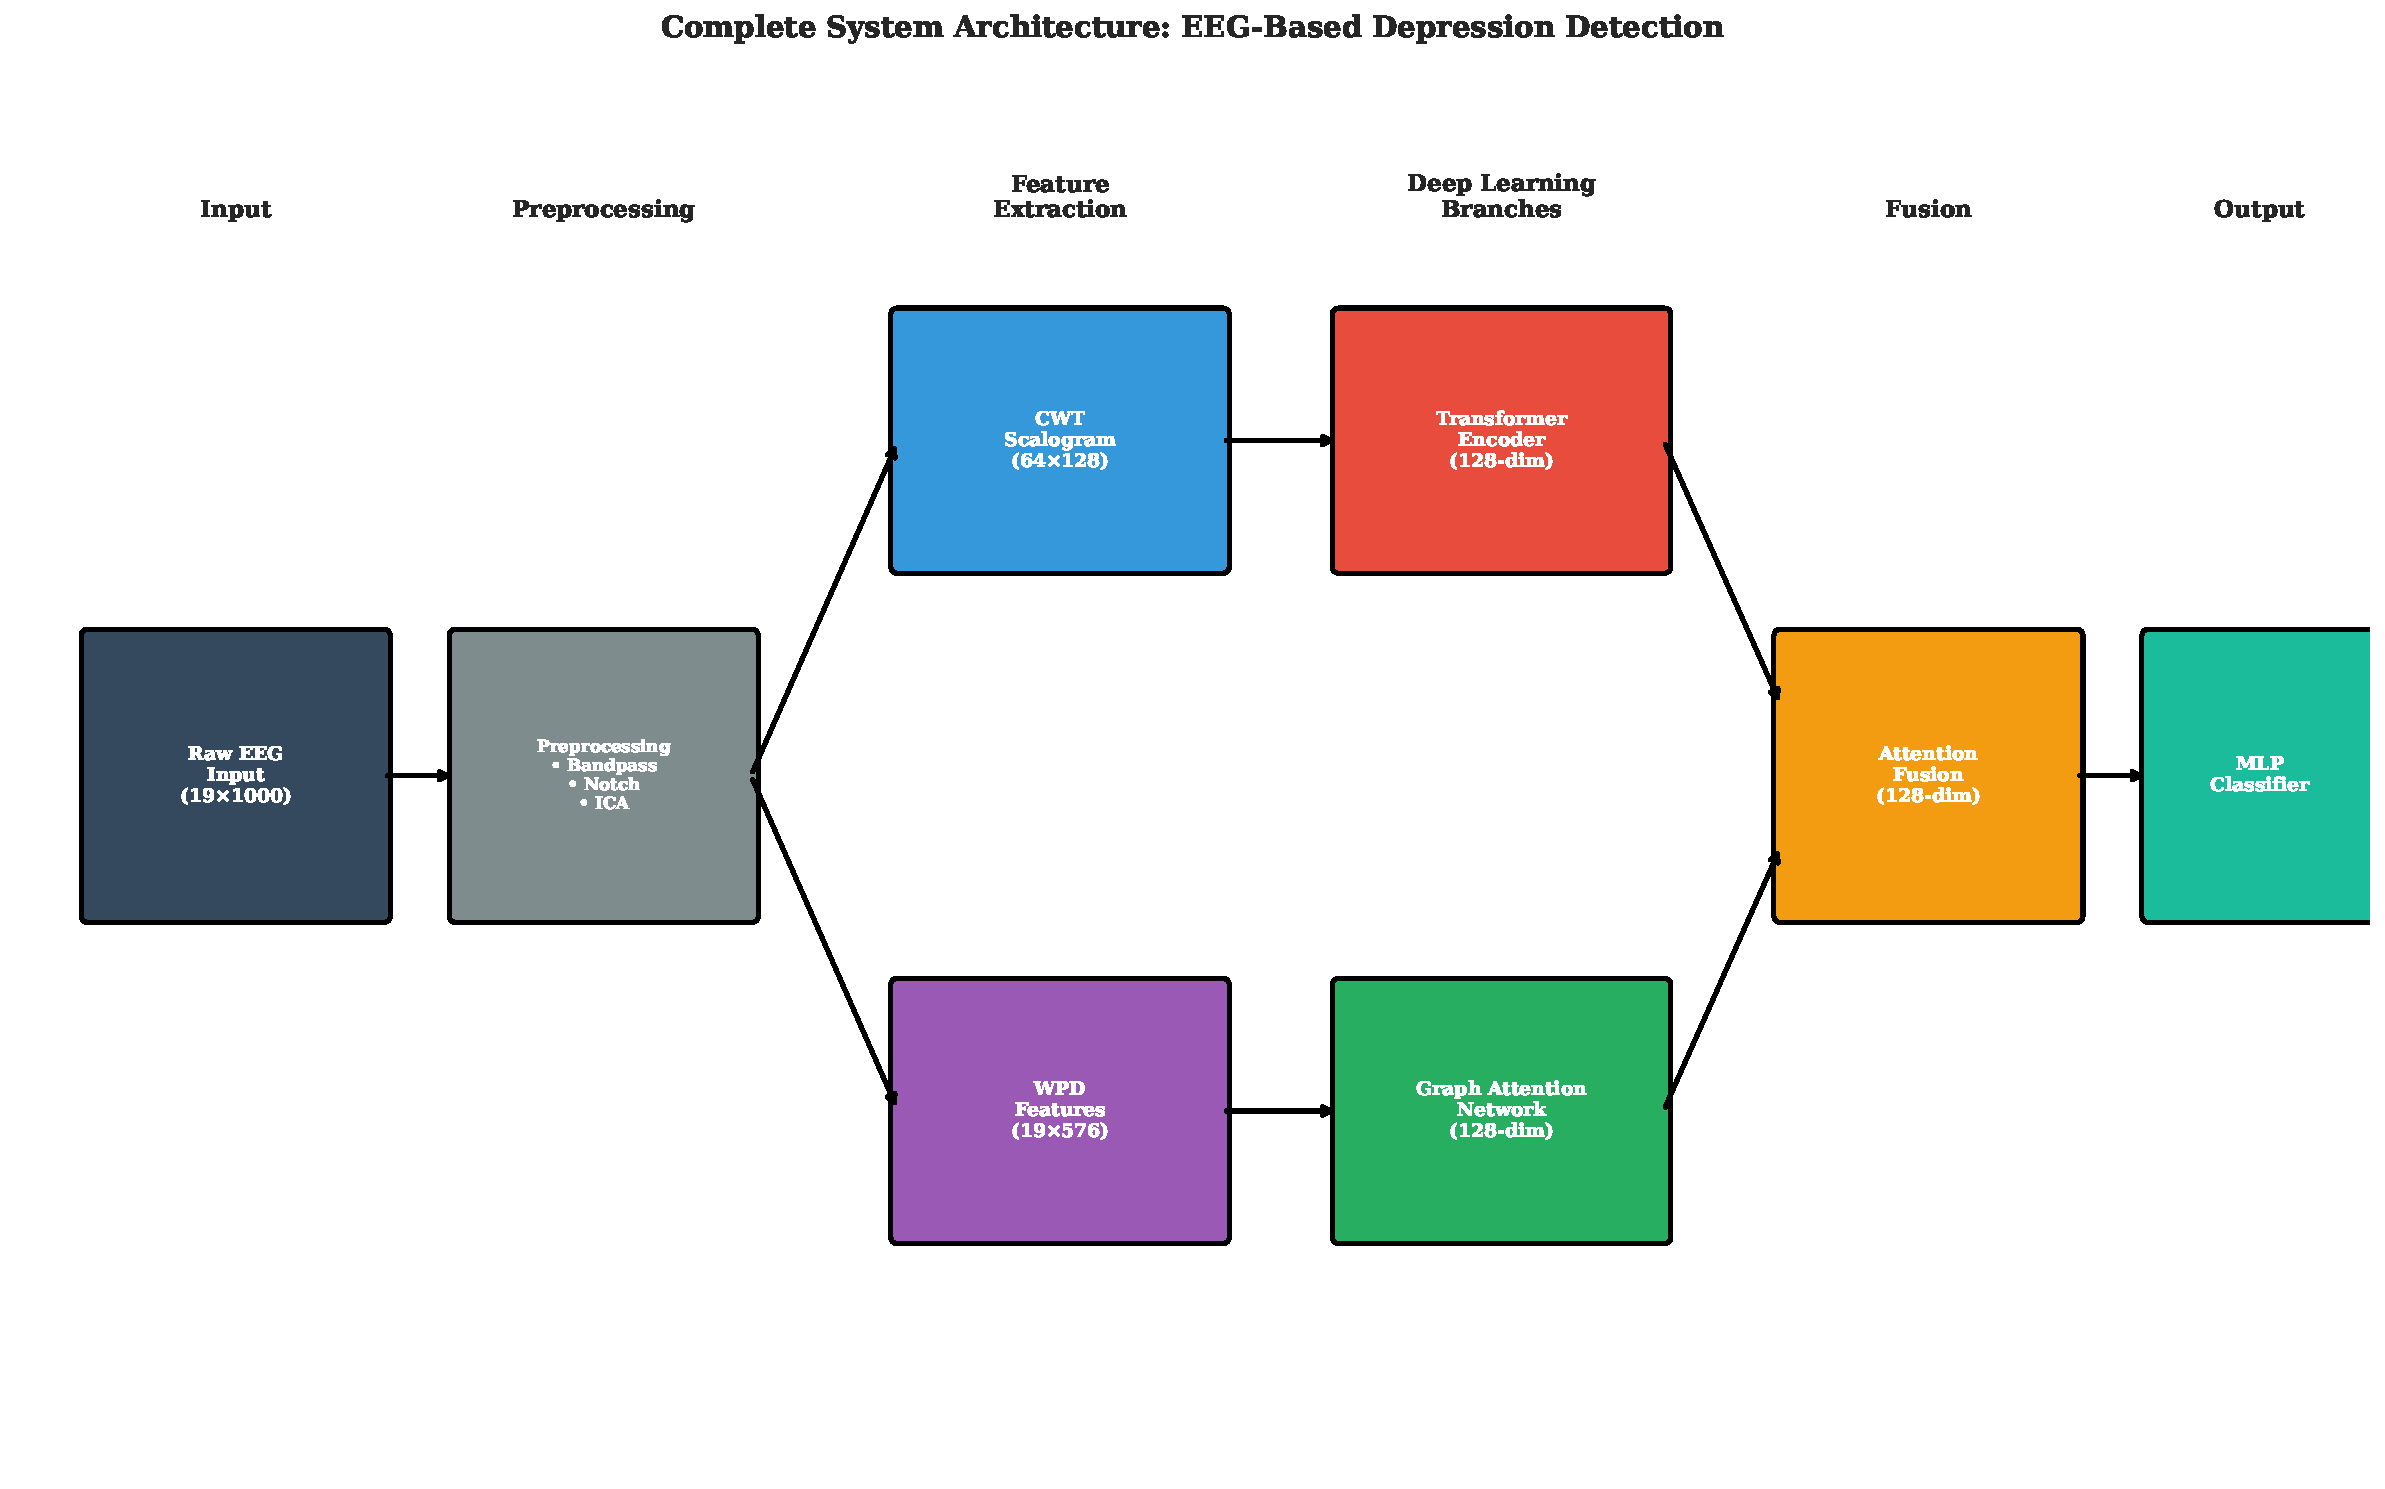
\includegraphics[width=0.95\textwidth]{figures/ch3/fig3_1_system_architecture.pdf}
    \caption{Complete system architecture showing the end-to-end processing pipeline from raw EEG signals to classification and explainability outputs.}
    \label{fig:system_architecture}
\end{figure}

\subsection{Data Flow Architecture}

At the highest level of abstraction, the system functions as a single processing unit that receives raw EEG data from the dataset repository and produces classification results with accompanying explainability reports for the clinician or researcher. The external entities interacting with the system are the EEG Dataset, which serves as the data source providing raw recordings, and the User who receives the processed outputs including depression probability scores, confidence metrics, and biomarker-level interpretations.

Decomposing the system reveals four major processing stages that operate sequentially on the data. The Data Preprocessing stage receives raw EEG signals and produces filtered, segmented epochs stored in an intermediate data structure. The Feature Extraction stage transforms these epochs into both WPD feature vectors and CWT scalograms, which may be cached for efficiency during repeated training runs. The Model Inference stage loads trained model weights and processes the extracted features through the dual-branch architecture to produce classification predictions. Finally, the Explainability Analysis stage computes attribution maps and concept scores that explain the model's decision-making process.

\section{METHODOLOGY}

\subsection{Data Preprocessing}

The preprocessing pipeline transforms raw EEG signals into clean, standardized epochs suitable for feature extraction. This transformation is critical because raw EEG recordings contain various artifacts and noise sources that would confound the classification task if not properly addressed. The preprocessing stages are applied sequentially, with each step building on the output of the previous stage to progressively refine the signal quality.

\begin{figure}[H]
    \centering
    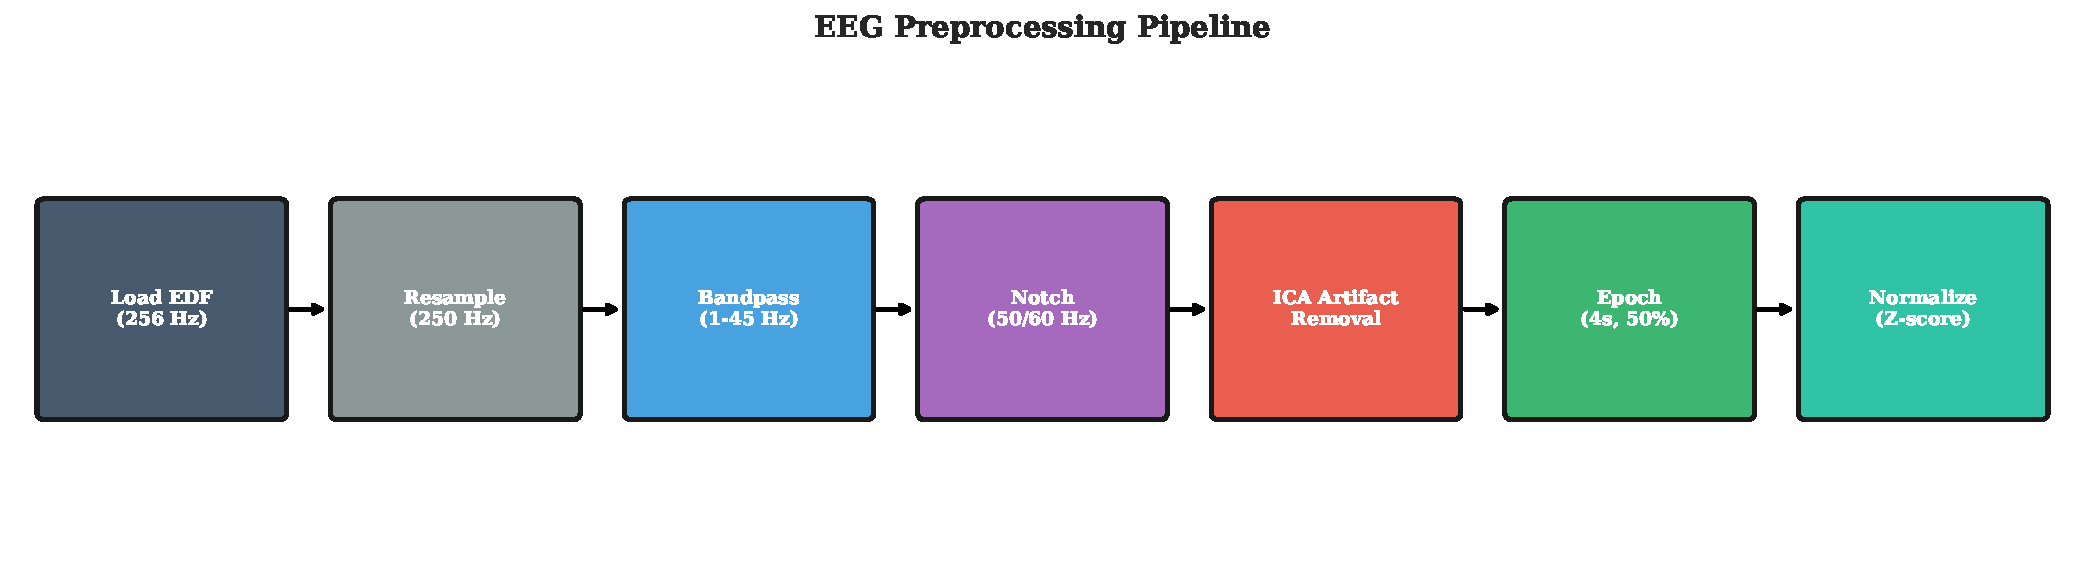
\includegraphics[width=0.95\textwidth]{figures/ch3/fig3_4_preprocessing.pdf}
    \caption{Preprocessing pipeline flowchart showing sequential signal processing stages.}
    \label{fig:preprocessing}
\end{figure}

\subsubsection{Filtering Operations}

The filtering stage applies two types of frequency-selective filters to remove unwanted signal components while preserving the neural activity of interest. A bandpass filter with cutoff frequencies of 1 Hz and 45 Hz removes both low-frequency drift and high-frequency noise that fall outside the range of standard EEG frequency bands. This filter is implemented as a Finite Impulse Response (FIR) filter with order 101, which provides linear phase characteristics that preserve the temporal relationships within the signal. The 1 Hz lower cutoff removes DC offset and slow baseline drift caused by electrode polarization and movement artifacts, while the 45 Hz upper cutoff eliminates high-frequency muscle artifacts and environmental electromagnetic interference while preserving the full gamma band activity.

Following the bandpass filter, notch filters at 50 Hz and 60 Hz remove power line interference that commonly contaminates EEG recordings. The 50 Hz notch addresses the European power grid frequency, while the 60 Hz notch addresses the North American standard, ensuring the preprocessing pipeline works correctly for datasets recorded in different geographic regions. Each notch filter has a bandwidth of 2 Hz, narrow enough to precisely target the interference frequency while minimizing distortion to nearby frequency components of interest.

\subsubsection{Artifact Removal}

Independent Component Analysis using the Picard algorithm decomposes the multi-channel EEG signal into statistically independent components, enabling identification and removal of artifact sources while preserving neural signals. Ocular artifacts from eye movements and blinks produce distinctive spatial patterns with high amplitude at frontal electrodes, while muscular artifacts from facial tension or jaw clenching produce characteristic high-frequency broadband activity. The ICA algorithm separates these artifact sources from neural components based on their statistical independence.

Components identified as artifactual based on their correlation with reference EOG channels (correlation greater than 0.8) are automatically rejected, and the signal is reconstructed from the remaining components. This automated rejection procedure ensures consistent artifact removal across all subjects while avoiding the subjectivity inherent in manual artifact identification.

\subsubsection{Epoch Segmentation}

Continuous recordings are segmented into discrete epochs of 4 seconds duration, corresponding to 1000 samples at the resampled rate of 250 Hz. The 4-second epoch length represents a carefully chosen compromise between conflicting requirements. Longer epochs capture more cycles of slower rhythms such as delta (1-4 Hz) and theta (4-8 Hz), providing stable estimates of low-frequency power. However, shorter epochs yield more samples per subject, which is valuable for training data-hungry deep learning models. The 4-second duration captures approximately 4-16 cycles of delta activity and 16-32 cycles of theta activity, sufficient for reliable spectral estimation while producing approximately 150 epochs per subject.

Epochs are extracted with 50\% overlap, meaning each time point in the continuous recording contributes to two consecutive epochs except at the boundaries. This overlap increases the total number of training samples while maintaining reasonable independence between adjacent epochs. Finally, amplitude-based rejection removes epochs containing any sample exceeding 100 µV, eliminating residual artifacts that survived the ICA cleaning process.

Table \ref{tab:preprocessing_params} summarizes the complete preprocessing parameter configuration.

\begin{table}[H]
    \centering
    \small
    \caption{Preprocessing Parameters}
    \label{tab:preprocessing_params}
    \begin{tabularx}{\textwidth}{|L{3.5cm}|L{2.5cm}|X|}
        \hline
        \textbf{Parameter} & \textbf{Value} & \textbf{Justification} \\
        \hline
        Original Sampling Rate & 256 Hz & Dataset specification \\
        \hline
        Resampled Rate & 250 Hz & Convenient for epoch length \\
        \hline
        Bandpass Range & 1-45 Hz & Covers delta through gamma \\
        \hline
        Filter Type & FIR, order 101 & Linear phase, stable \\
        \hline
        Notch Frequencies & 50, 60 Hz & Power line removal \\
        \hline
        ICA Algorithm & Picard & Fast, reliable \\
        \hline
        Epoch Duration & 4 seconds & Sufficient for slow rhythms \\
        \hline
        Epoch Overlap & 50\% & Balance data quantity and independence \\
        \hline
        Amplitude Threshold & 100 $\mu$V & Artifact rejection \\
        \hline
    \end{tabularx}
\end{table}

\subsection{Feature Extraction}

The system extracts two complementary feature types that capture different aspects of the EEG signal. Wavelet Packet Decomposition features provide fine-grained spectral analysis with 576 features per channel, serving as node attributes for the Graph Attention Network branch. Continuous Wavelet Transform scalograms provide two-dimensional time-frequency representations that serve as input to the Vision Transformer branch. This dual-feature approach ensures that both branches receive inputs optimized for their respective architectures.

\subsubsection{Wavelet Packet Decomposition (WPD)}

Wavelet Packet Decomposition extends the standard discrete wavelet transform by recursively decomposing both approximation and detail coefficients at each level, providing uniform frequency resolution across the entire spectrum. Unlike the standard DWT which only decomposes the low-frequency approximation coefficients, WPD treats approximation and detail coefficients symmetrically, yielding a complete binary tree of frequency subbands.

\begin{figure}[H]
    \centering
    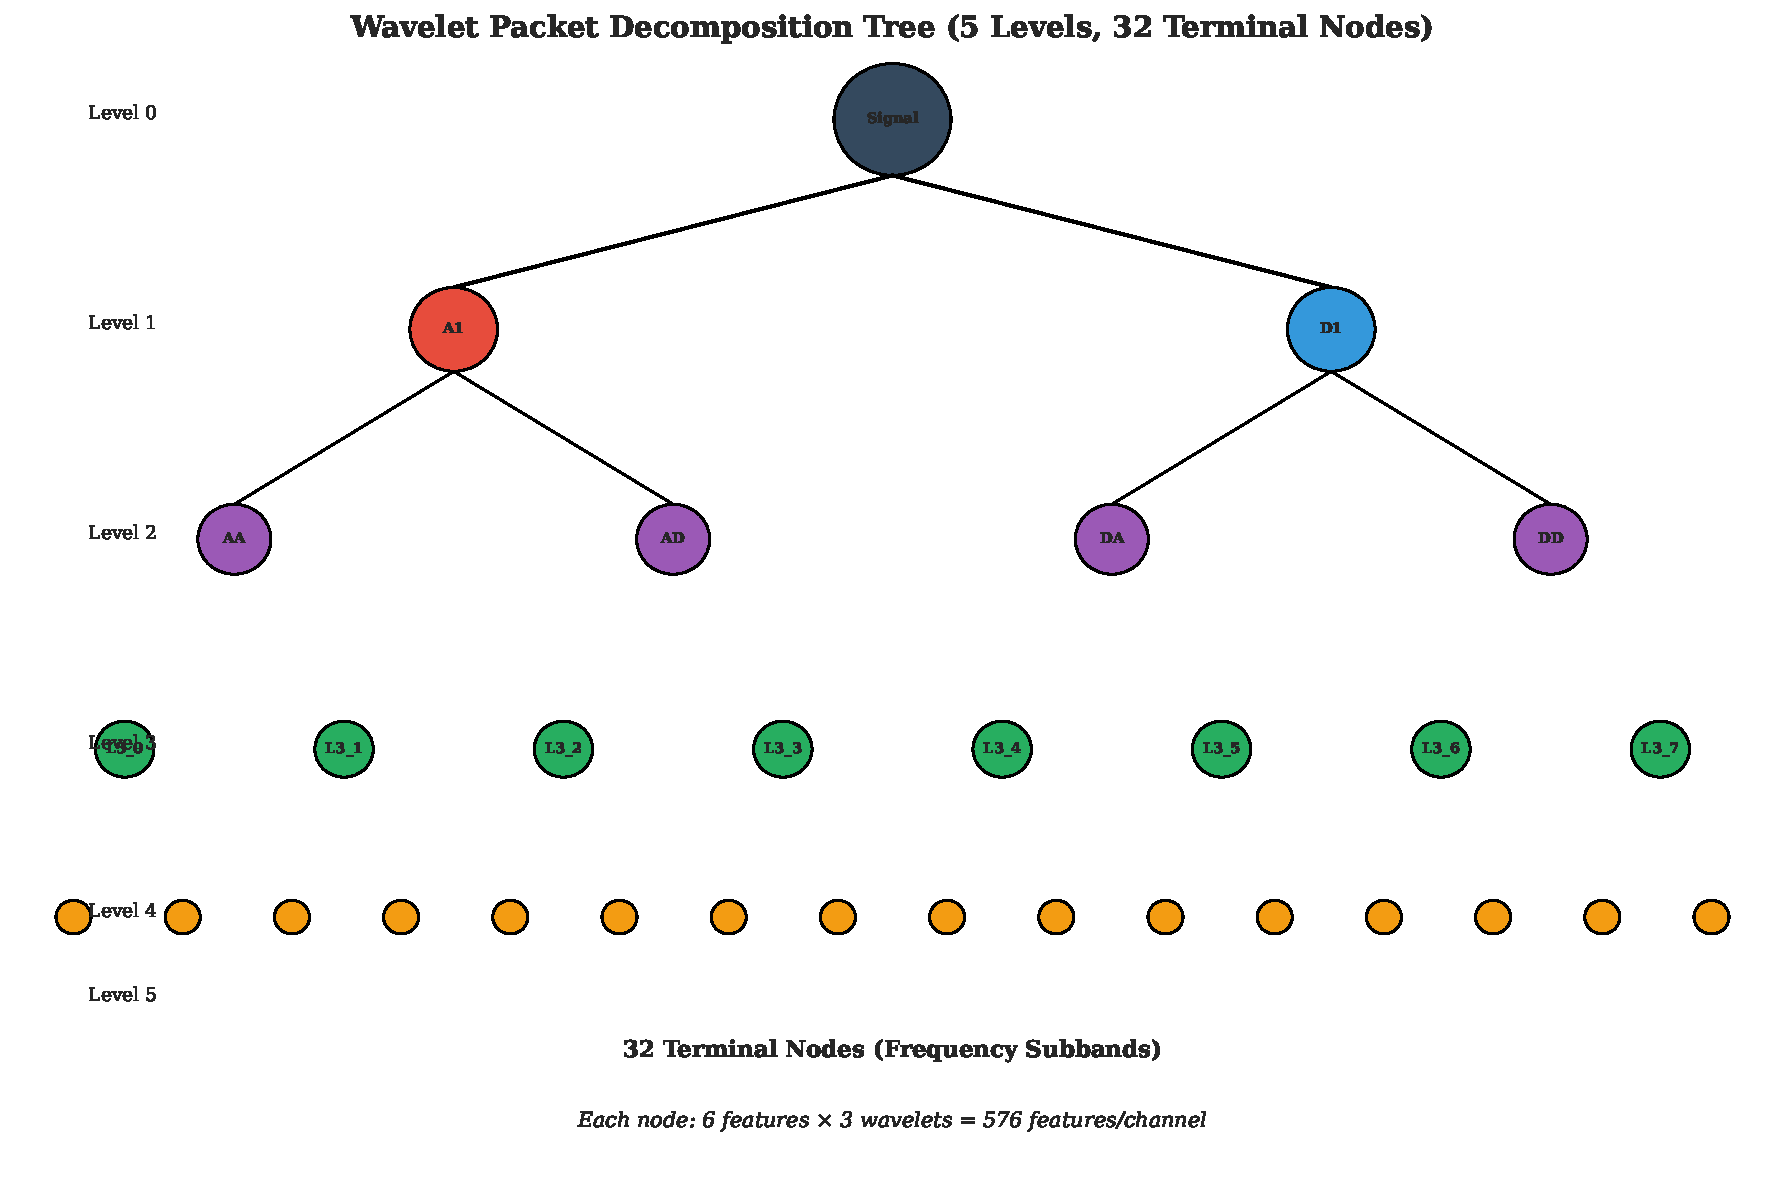
\includegraphics[width=0.95\textwidth]{figures/ch3/fig3_5_wpd_tree.pdf}
    \caption{Wavelet Packet Decomposition tree showing 5-level decomposition into 32 frequency subbands.}
    \label{fig:wpd_tree}
\end{figure}

The multi-wavelet approach employed in this system uses three complementary wavelet families rather than a single wavelet, capturing different signal characteristics through their distinct mathematical properties. The Daubechies-4 (db4) wavelet offers good time-frequency localization with a waveform shape similar to neural transients, making it well-suited for detecting sharp features in EEG signals. The Symlet-5 (sym5) wavelet provides near-symmetric filter coefficients with smooth oscillatory characteristics, reducing boundary effects at epoch edges and capturing sustained rhythmic activity. The Coiflet-3 (coif3) wavelet offers excellent symmetry with high-order vanishing moments, enabling accurate representation of polynomial trends and slowly-varying signal components.

For each of the 32 terminal nodes in the WPD tree, six statistical features are computed to characterize the coefficient distribution. Energy, computed as the sum of squared coefficients, measures the total power in each frequency subband and directly relates to traditional spectral power measures. Shannon entropy quantifies signal complexity and irregularity, with higher values indicating more random or unpredictable coefficient distributions. Log energy entropy provides an alternative complexity measure with different sensitivity characteristics. The mean captures any DC offset in the coefficient distribution, while standard deviation measures the variability around that mean. Skewness, the third standardized moment, characterizes the asymmetry of the coefficient distribution.

The total feature dimensionality per channel is computed as the product of three wavelets, 32 terminal nodes, and 6 features, yielding 576 features per channel. With 19 EEG channels, the complete WPD feature vector contains 10,944 elements, providing a rich spectral representation that captures fine-grained frequency information across the entire EEG spectrum.

\begin{table}[H]
    \centering
    \small
    \caption{WPD Feature Extraction Parameters}
    \label{tab:wpd_params}
    \begin{tabularx}{\textwidth}{|L{3.5cm}|L{3cm}|X|}
        \hline
        \textbf{Parameter} & \textbf{Value} & \textbf{Description} \\
        \hline
        Wavelet Families & db4, sym5, coif3 & Complementary characteristics \\
        \hline
        Decomposition Level & 5 & Yields 32 terminal nodes \\
        \hline
        Terminal Nodes & 32 per wavelet & Frequency resolution $\approx$ 3.9 Hz \\
        \hline
        Features per Node & 6 & Energy, entropy, statistics \\
        \hline
        Features per Channel & 576 & 3 $\times$ 32 $\times$ 6 \\
        \hline
        Total Features & 10,944 & 19 channels $\times$ 576 features \\
        \hline
    \end{tabularx}
\end{table}

\subsubsection{Continuous Wavelet Transform (CWT)}

The Continuous Wavelet Transform generates a two-dimensional time-frequency representation called a scalogram that encodes how the spectral content of the signal evolves over time. Unlike the discrete decomposition provided by WPD, CWT computes wavelet coefficients at all scales and time points, producing a dense image-like representation ideal for processing with convolutional or attention-based architectures.

\begin{figure}[H]
    \centering
    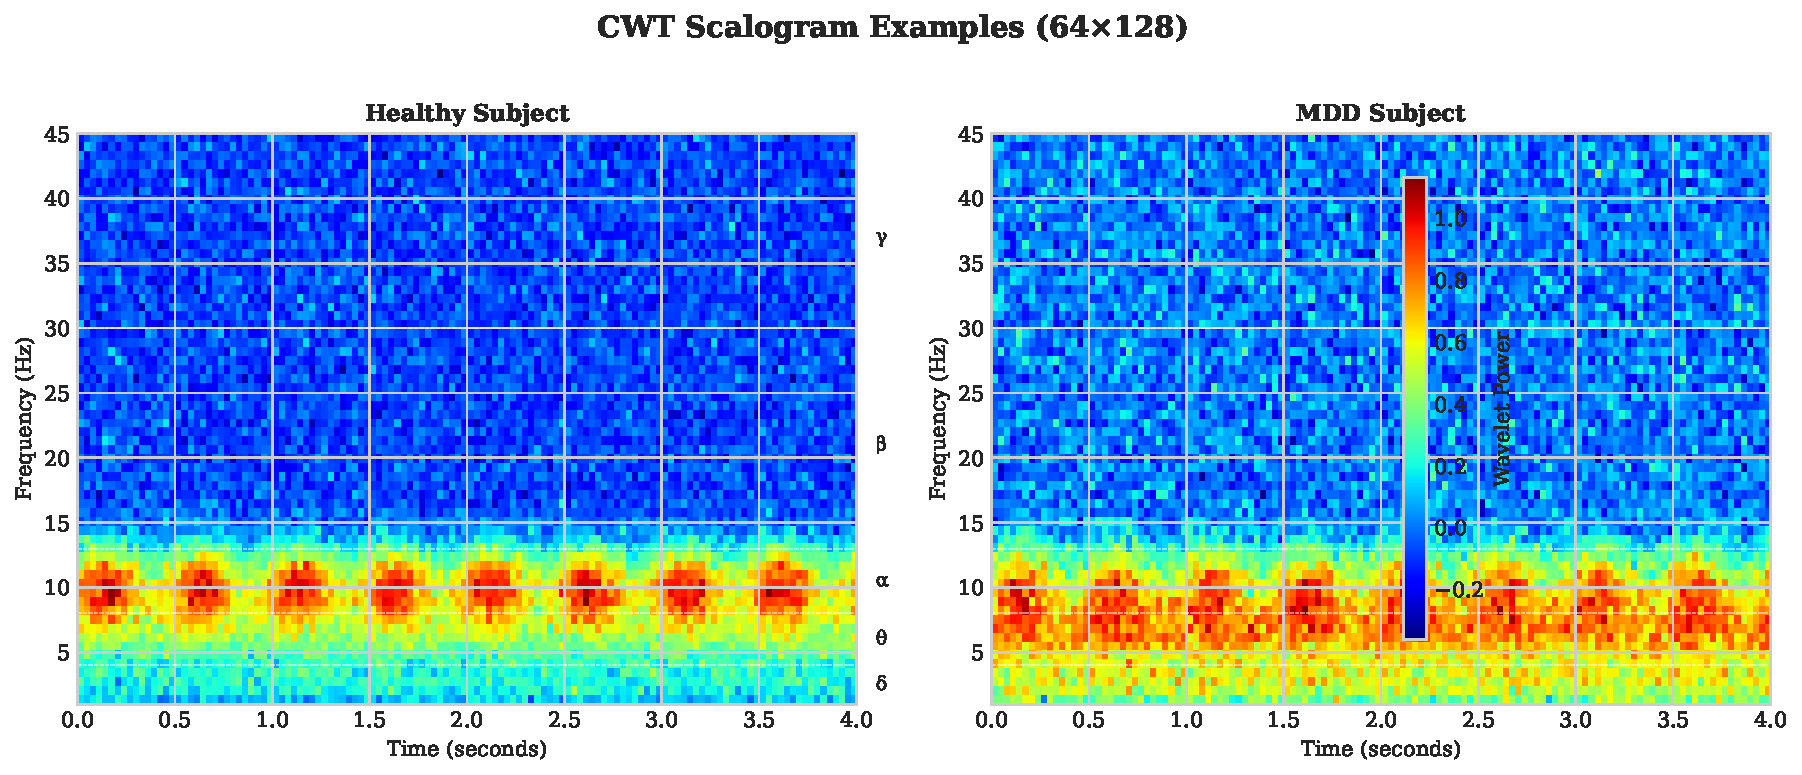
\includegraphics[width=0.85\textwidth]{figures/ch3/fig3_6_cwt_scalogram.pdf}
    \caption{Example CWT scalogram showing time-frequency representation of a 4-second EEG epoch. Horizontal bands indicate dominant frequency components; vertical patterns show temporal dynamics.}
    \label{fig:cwt_scalogram}
\end{figure}

The Complex Morlet wavelet with bandwidth parameter 1.5 and center frequency 1.0 serves as the analyzing wavelet, providing an excellent balance between time and frequency resolution for EEG analysis. The complex-valued wavelet yields both magnitude and phase information, though for the current implementation only magnitude is used. The output scalogram spans frequencies from 1 Hz to 45 Hz using 64 logarithmically-spaced frequency bins, capturing the full range of clinically relevant EEG activity from delta through gamma bands. The temporal dimension contains 128 time points spanning the 4-second epoch, yielding a final scalogram shape of 64 rows (frequency) by 128 columns (time) per channel. For computational efficiency, the scalograms are averaged across channels to produce a single representative time-frequency image per epoch.

\subsection{Model Architecture}

The proposed model consists of three main components that work together to produce depression classifications: the Transformer Branch processes time-frequency representations, the GNN Branch processes spatial electrode relationships, and the Attention-Based Fusion module combines their outputs.

\subsubsection{Transformer Branch}

The Transformer Branch processes CWT scalograms using a Vision Transformer architecture adapted for time-frequency analysis of EEG signals. The Vision Transformer, originally developed for image classification, treats two-dimensional inputs as sequences of patches and applies self-attention to learn global dependencies between patch locations. This approach is well-suited for scalogram processing because depression-related patterns may involve interactions between distant time-frequency regions that local convolutional receptive fields would miss.

\begin{figure}[H]
    \centering
    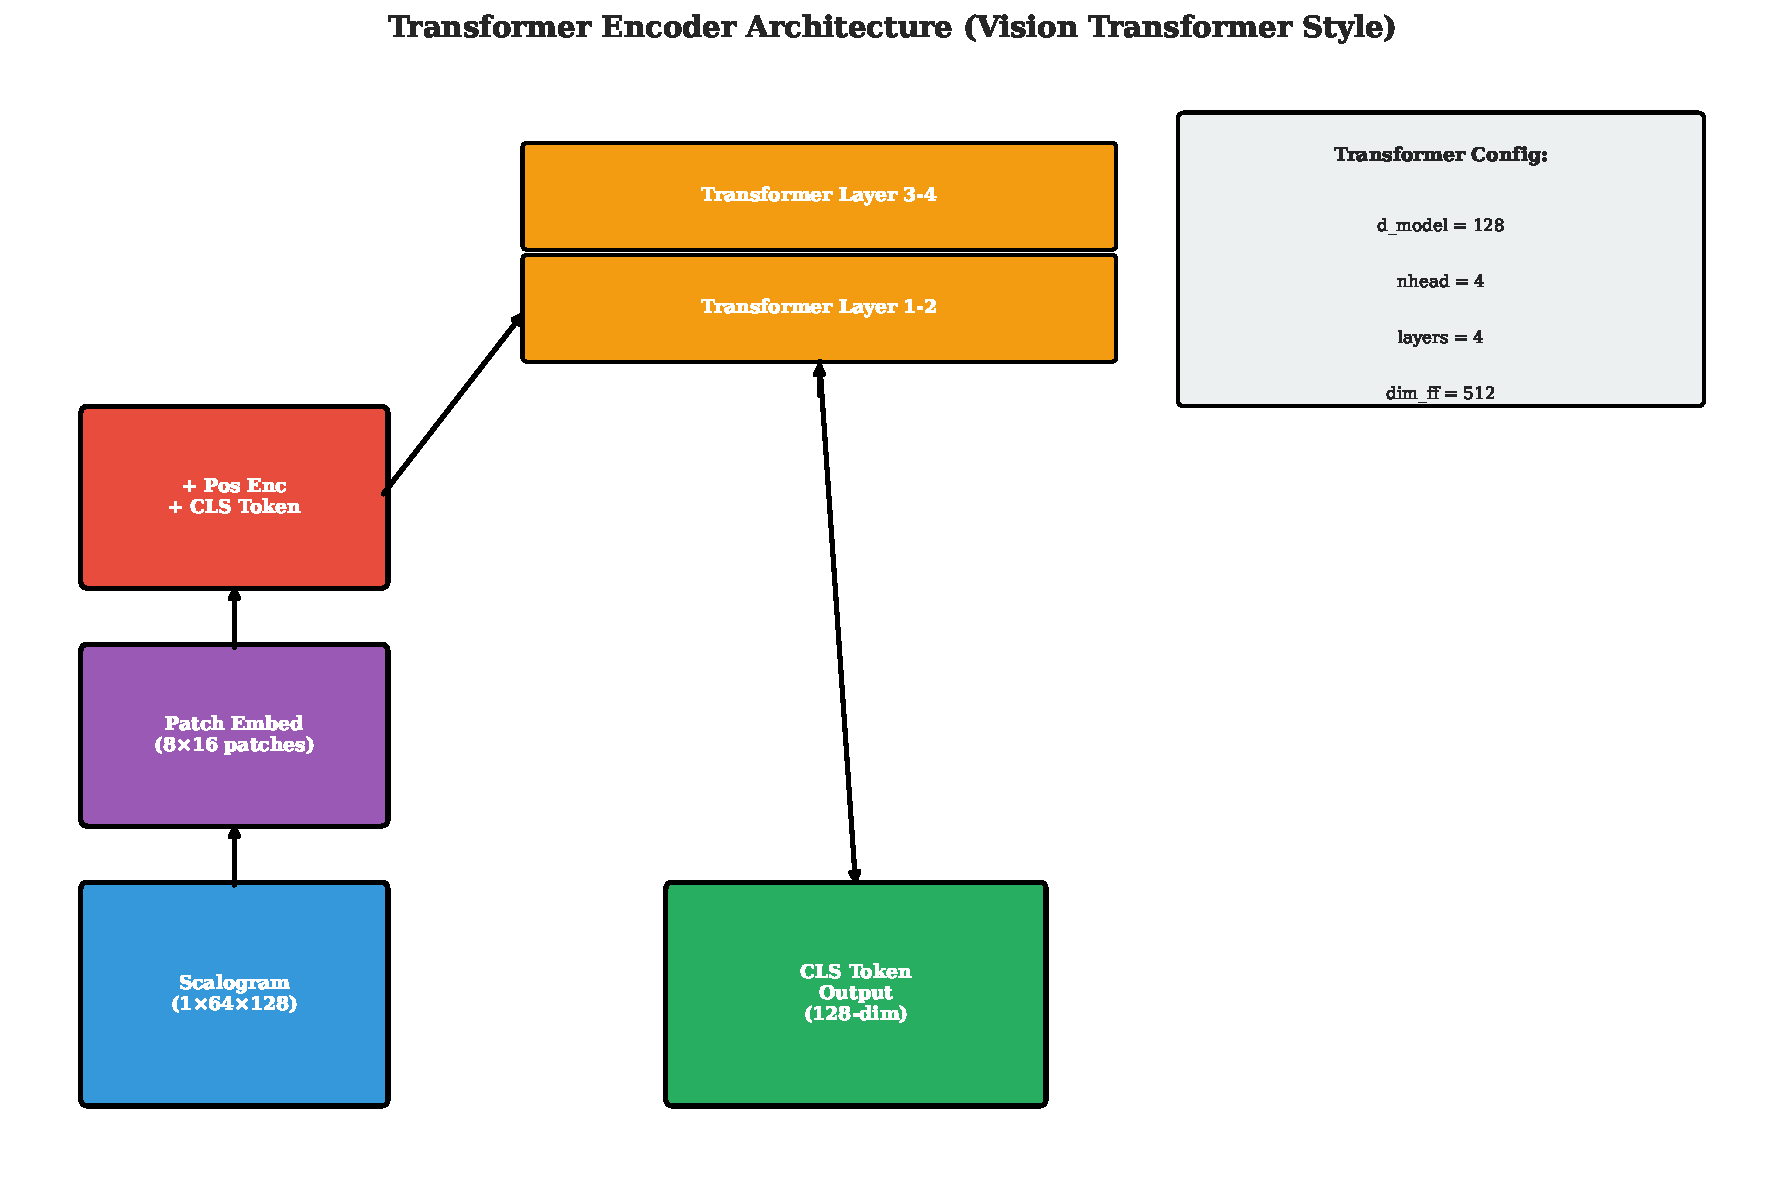
\includegraphics[width=0.95\textwidth]{figures/ch3/fig3_7_transformer.pdf}
    \caption{Transformer encoder architecture for processing CWT scalograms, following Vision Transformer design principles.}
    \label{fig:transformer_arch}
\end{figure}

The input scalogram of size 64×128 is divided into non-overlapping patches of size 8×16, yielding 64 patches that tile the complete time-frequency plane. Each patch is flattened and linearly projected to the model dimension of 128, converting the 128-element patch into a 128-dimensional embedding vector. This projection is learned during training, allowing the model to discover optimal low-dimensional representations of local time-frequency regions.

Learnable positional embeddings are added to the patch embeddings to preserve information about where each patch was located in the original scalogram. Without positional encoding, the Transformer would be permutation-invariant and unable to distinguish whether a particular pattern occurred early or late in the epoch, or in low versus high frequency regions. A learnable classification token is prepended to the sequence of patch embeddings, serving as an aggregation point that collects information from all patches through the attention mechanism.

The resulting sequence of 65 tokens (64 patches plus the CLS token) passes through four Transformer encoder layers, each containing multi-head self-attention followed by a feed-forward network with GELU activation. The self-attention mechanism with 4 heads allows each position to attend to all other positions, learning which time-frequency regions are most relevant to each other for depression detection. After processing through all encoder layers, the final representation of the CLS token serves as the 128-dimensional output of the Transformer branch.

\begin{table}[H]
    \centering
    \small
    \caption{Transformer Branch Hyperparameters}
    \label{tab:transformer_params}
    \begin{tabularx}{\textwidth}{|L{4cm}|L{2.5cm}|X|}
        \hline
        \textbf{Parameter} & \textbf{Value} & \textbf{Rationale} \\
        \hline
        Input Size & 64 $\times$ 128 & CWT scalogram dimensions \\
        \hline
        Patch Size & 8 $\times$ 16 & 64 total patches \\
        \hline
        Model Dimension (d\_model) & 128 & Memory efficient; expressive \\
        \hline
        Attention Heads & 4 & Head dimension = 32 \\
        \hline
        Encoder Layers & 4 & Sufficient depth for patterns \\
        \hline
        Feed-Forward Dimension & 512 & 4$\times$ d\_model (standard) \\
        \hline
        Dropout & 0.1 & Regularization \\
        \hline
        Activation & GELU & Smooth, works well with Transformers \\
        \hline
        Use CLS Token & True & Classification representation \\
        \hline
        Output Dimension & 128 & Matches d\_model \\
        \hline
        Parameters & 892,416 & Transformer branch total \\
        \hline
    \end{tabularx}
\end{table}

\subsubsection{GNN Branch}

The Graph Attention Network branch models spatial relationships between EEG electrodes by representing them as nodes in a graph where edges encode connectivity patterns. Unlike approaches that treat EEG channels as independent features or as a simple sequence, the GNN explicitly captures the topological structure of the electrode array and learns which inter-electrode relationships are most informative for depression detection.

\begin{figure}[H]
    \centering
    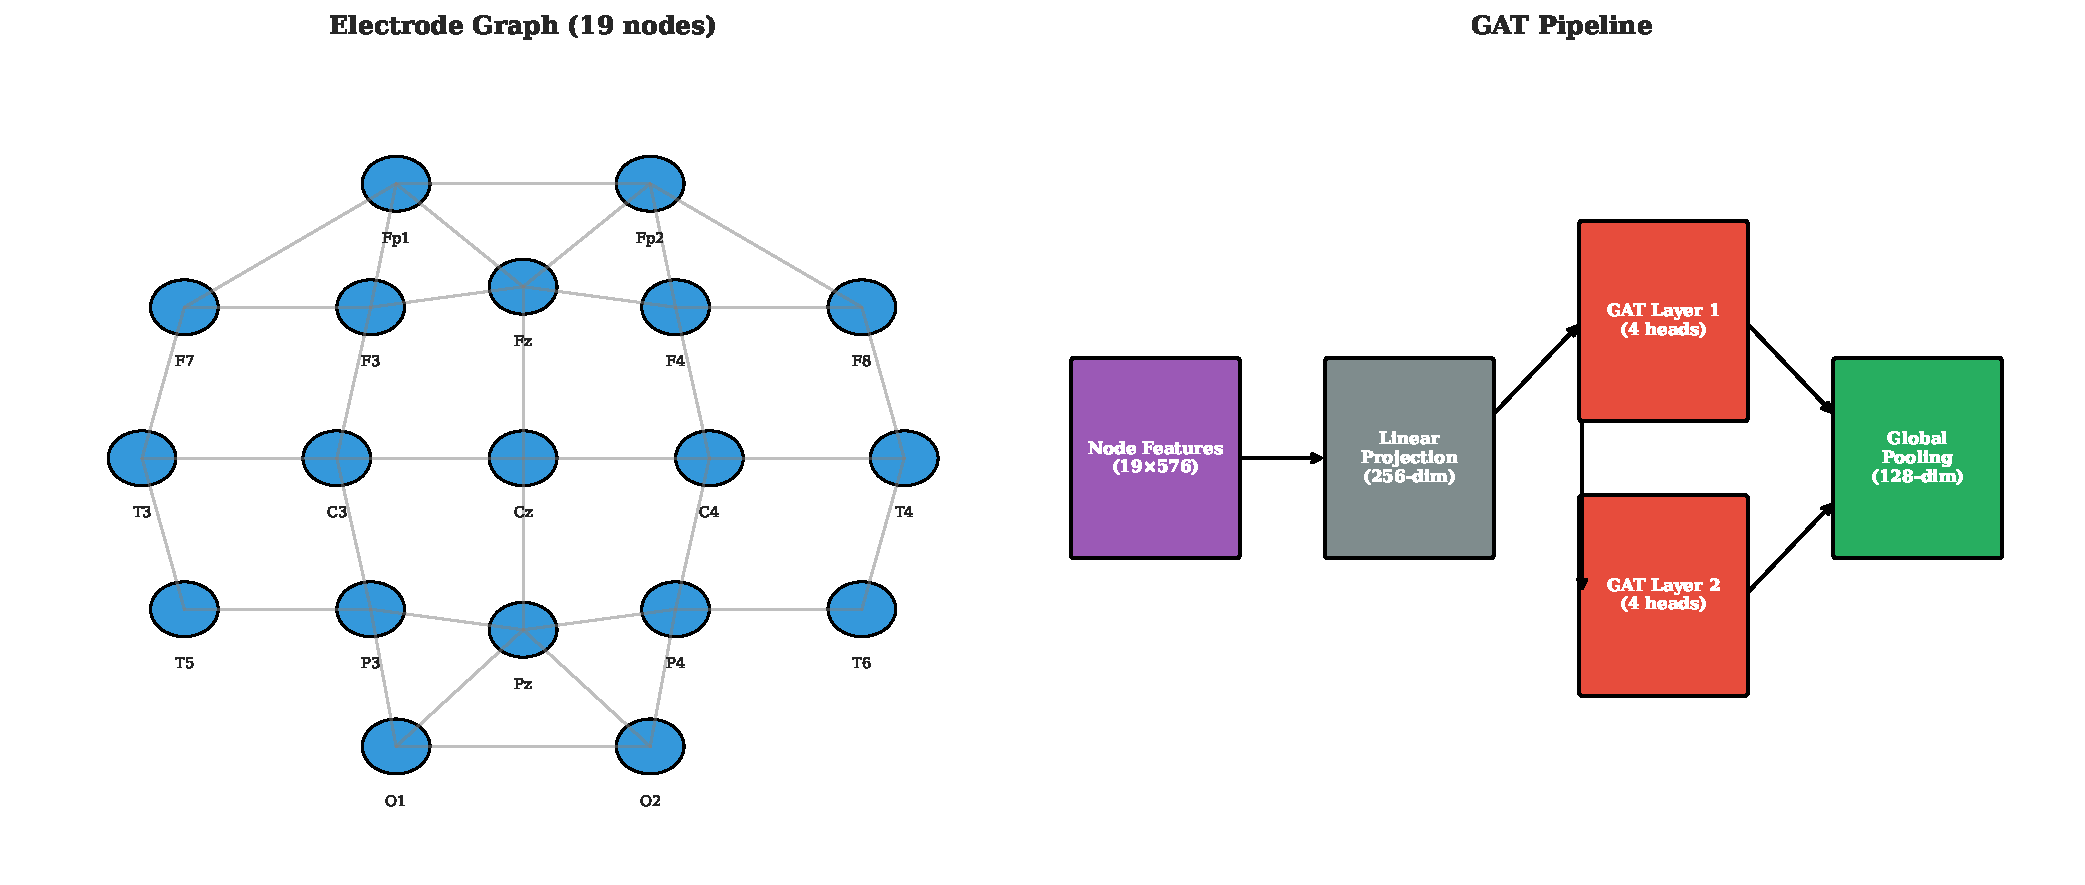
\includegraphics[width=0.95\textwidth]{figures/ch3/fig3_8_gnn.pdf}
    \caption{Graph Attention Network architecture showing electrode graph construction and message passing layers.}
    \label{fig:gnn_arch}
\end{figure}

The electrode graph is constructed using a hybrid adjacency scheme that combines spatial proximity with functional connectivity. The spatial adjacency component connects each electrode to its 6 nearest neighbors based on the three-dimensional coordinates of the 10-20 electrode positions, capturing the physical layout of the recording array. The functional adjacency component adds edges between electrode pairs whose signals show Pearson correlation exceeding 0.5, capturing data-driven connectivity patterns that may reflect underlying neural coupling. This hybrid approach ensures that both anatomically-grounded and functionally-observed relationships inform the graph structure.

Each node in the graph receives the 576-dimensional WPD feature vector computed for the corresponding electrode as its input attribute. An initial projection layer reduces this to a 256-dimensional hidden representation. Three Graph Attention convolutional layers then perform message passing, where each node aggregates information from its neighbors weighted by learned attention coefficients. The attention mechanism enables the network to focus on the most relevant connections for depression detection, providing interpretability through the learned attention weights. Multi-head attention with 4 heads allows the network to attend to different aspects of the connectivity patterns simultaneously.

After the final GAT layer, global mean pooling aggregates node representations across the entire graph into a single 128-dimensional vector, producing an output that matches the dimensionality of the Transformer branch for fusion.

\begin{table}[H]
    \centering
    \small
    \caption{GNN Branch Hyperparameters}
    \label{tab:gnn_params}
    \begin{tabularx}{\textwidth}{|L{4cm}|L{2.5cm}|X|}
        \hline
        \textbf{Parameter} & \textbf{Value} & \textbf{Rationale} \\
        \hline
        Number of Nodes & 19 & 10-20 electrode montage \\
        \hline
        Node Feature Dimension & 576 & WPD features per channel \\
        \hline
        Hidden Dimension & 256 & Intermediate representation \\
        \hline
        Output Dimension & 128 & Matches Transformer output \\
        \hline
        GAT Layers & 3 & Sufficient for 19-node graph \\
        \hline
        Attention Heads & 4 & Multi-head attention \\
        \hline
        Spatial k-neighbors & 6 & Local connectivity \\
        \hline
        Functional Threshold & 0.5 & Correlation-based edges \\
        \hline
        Dropout & 0.3 & Higher than Transformer (smaller graph) \\
        \hline
        Pooling & Global Mean & Aggregate node features \\
        \hline
        Parameters & 462,592 & GNN branch total \\
        \hline
    \end{tabularx}
\end{table}

\subsubsection{Attention-Based Fusion}

The fusion module adaptively combines the 128-dimensional feature vectors from the Transformer and GNN branches, learning to weight their contributions based on the input characteristics. Simple concatenation or averaging would treat both branches equally regardless of which provides more relevant information for a particular sample. The attention-based approach instead learns dynamic weights that can emphasize whichever modality is more informative.

The cross-attention mechanism enables each branch to attend to the other, learning which complementary features to incorporate. When the Transformer features attend to the GNN features, the model learns which spatial connectivity patterns are most relevant given the observed time-frequency characteristics. Conversely, when the GNN features attend to the Transformer features, the model learns which time-frequency patterns matter most given the spatial electrode relationships. This bidirectional attention creates a rich interaction between the two modalities.

Learned gating weights further modulate the branch contributions, computed by a small neural network that receives the concatenated branch outputs and produces a two-element softmax-normalized weight vector. These weights determine the relative contribution of each branch to the final fused representation. The output projection combines the attended features with the gated mixture, producing a 128-dimensional fused representation that proceeds to the classification head.

\subsection{Training Strategy}

\subsubsection{LOSO Cross-Validation}

Leave-One-Subject-Out cross-validation ensures honest performance evaluation by completely separating subjects between training and test sets. The protocol iterates through all 58 subjects, holding out one subject at a time as the test set while training on the remaining 57 subjects. This creates 58 independent training runs, each evaluated on a subject whose data was never seen during training.

\begin{figure}[H]
    \centering
    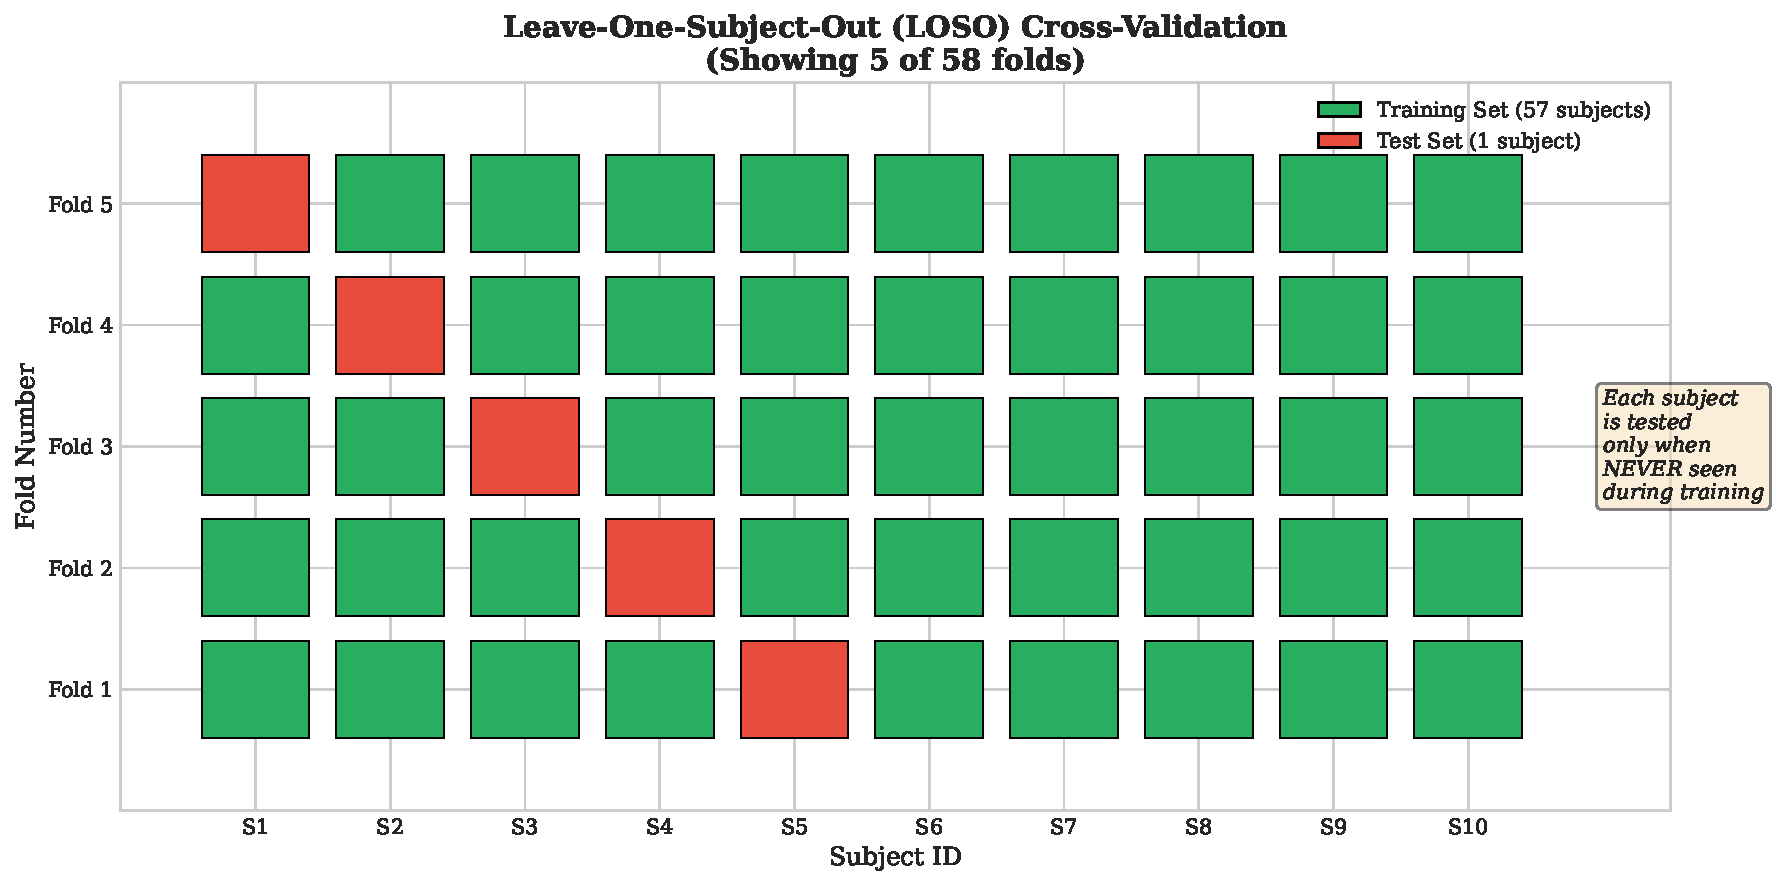
\includegraphics[width=0.9\textwidth]{figures/ch3/fig3_10_loso.pdf}
    \caption{Leave-One-Subject-Out (LOSO) cross-validation protocol ensuring each subject is tested only when completely unseen during training.}
    \label{fig:loso}
\end{figure}

For each fold, the held-out subject's epochs form the test set, while the remaining subjects are further split into training and validation sets using a 90/10 split. The model is trained from scratch with random initialization, as transfer learning between folds could introduce subtle information leakage. Training proceeds for up to 30 epochs with early stopping based on validation loss with patience of 10 epochs, preventing overfitting while allowing sufficient training when validation performance continues improving. After training completes, the model is evaluated on the test subject and predictions are saved along with ground truth labels for later aggregation.

After completing all 58 folds, the predictions are aggregated to compute final performance metrics. Subject-level accuracy is computed by majority voting across each subject's epochs, while sample-level accuracy is computed across all individual epoch predictions. Additional metrics including AUC-ROC, F1-score, precision, recall, and confusion matrix provide a comprehensive view of classification performance.

\begin{table}[H]
    \centering
    \small
    \caption{Training Configuration}
    \label{tab:training_config}
    \begin{tabularx}{\textwidth}{|L{3.5cm}|L{3cm}|X|}
        \hline
        \textbf{Parameter} & \textbf{Value} & \textbf{Description} \\
        \hline
        Cross-Validation & LOSO & 58 folds (one per subject) \\
        \hline
        Epochs per Fold & 30 & With early stopping \\
        \hline
        Batch Size & 16 & Limited by GPU memory \\
        \hline
        Effective Batch & 32 & Via gradient accumulation (2 steps) \\
        \hline
        Optimizer & AdamW & Decoupled weight decay \\
        \hline
        Learning Rate & 1e-4 & Conservative for small dataset \\
        \hline
        Weight Decay & 0.01 & L2 regularization \\
        \hline
        Scheduler & CosineAnnealing & With warm restarts \\
        \hline
        Early Stopping & Patience 10 & Prevent overfitting \\
        \hline
        Mixed Precision & FP16 & Memory efficiency \\
        \hline
        Gradient Clipping & 1.0 & Training stability \\
        \hline
    \end{tabularx}
\end{table}

\section{MODULE DESCRIPTION}

The system is organized into nine modules with clearly defined responsibilities and interfaces. Table \ref{tab:modules} describes each module with its input and output specifications, enabling independent development, testing, and maintenance of system components.

\begin{table}[H]
    \centering
    \small
    \caption{Module Input/Output Specifications}
    \label{tab:modules}
    \begin{tabularx}{\textwidth}{|L{2cm}|L{3cm}|L{3cm}|X|}
        \hline
        \textbf{Module} & \textbf{Input} & \textbf{Output} & \textbf{Function} \\
        \hline
        M1: Data Loading & EDF file paths & Raw EEG arrays (19, N) & Load multi-channel recordings \\
        \hline
        M2: Preprocessing & Raw EEG (19, N) & Filtered epochs (B, 19, 1000) & Filter, segment, normalize \\
        \hline
        M3: WPD Extraction & Epochs (B, 19, 1000) & WPD features (B, 19, 576) & Multi-wavelet decomposition \\
        \hline
        M4: CWT Generation & Epochs (B, 19, 1000) & Scalograms (B, 1, 64, 128) & Time-frequency transform \\
        \hline
        M5: Transformer & Scalogram (B, 1, 64, 128) & Features (B, 128) & Time-frequency encoding \\
        \hline
        M6: GNN & WPD (B, 19, 576), Graph & Features (B, 128) & Spatial encoding \\
        \hline
        M7: Fusion & Trans (B, 128), GNN (B, 128) & Fused (B, 128) & Feature combination \\
        \hline
        M8: Classifier & Fused (B, 128) & Probability (B, 1) & Depression prediction \\
        \hline
        M9: Explainability & Model, Input & Attributions, Scores & IG, LRP, TCAV \\
        \hline
    \end{tabularx}
\end{table}

The data flow between modules follows a logical progression from raw data to final predictions. The Data Loading module (M1) parses EDF files and extracts multi-channel time series. The Preprocessing module (M2) applies filtering and segmentation to produce standardized epochs. The WPD Extraction (M3) and CWT Generation (M4) modules operate in parallel on the preprocessed epochs, producing features for their respective model branches. The Transformer (M5) and GNN (M6) modules encode their inputs into fixed-dimensional representations. The Fusion module (M7) combines branch outputs, and the Classifier (M8) produces final predictions. The Explainability module (M9) operates after training to analyze model decision-making through gradient-based and concept-based methods.

\section{DATA DESIGN}

\subsection{Dataset Specification}

The system uses the Figshare MDD EEG Dataset, a publicly available resource specifically curated for depression research. This dataset provides resting-state EEG recordings from both Major Depressive Disorder patients and healthy control subjects, recorded under standardized conditions that ensure comparability across subjects.

The dataset is organized into two subdirectories corresponding to the two diagnostic categories. The MDD directory contains 29 recordings from patients diagnosed with Major Depressive Disorder according to DSM-5 criteria, while the Healthy directory contains 29 recordings from control subjects with no psychiatric history. Each recording file follows a standardized naming convention indicating the diagnostic group, subject number, and recording condition (Eyes Closed). The Eyes Closed resting state condition was chosen because it minimizes visual processing artifacts while maintaining a standardized cognitive state across subjects.

\subsection{Dataset Demographics}

The dataset includes balanced representation of both diagnostic groups with matched demographic characteristics to minimize confounding variables. Table \ref{tab:demographics} presents the demographic characteristics of the participant groups.

\begin{table}[H]
    \centering
    \small
    \caption{Dataset Demographics}
    \label{tab:demographics}
    \begin{tabularx}{\textwidth}{|X|c|c|}
        \hline
        \textbf{Characteristic} & \textbf{MDD Group} & \textbf{Healthy Control} \\
        \hline
        Number of Subjects & 29 & 29 \\
        \hline
        Age Range & 18-65 years & 18-65 years \\
        \hline
        Gender & Mixed & Mixed \\
        \hline
        Diagnosis & DSM-5 MDD criteria & No psychiatric history \\
        \hline
        Medication Status & Medication-free or stable & None \\
        \hline
    \end{tabularx}
\end{table}

\subsection{Recording Parameters}

All recordings follow the International 10-20 System for electrode placement, using 19 standard electrode positions that provide comprehensive coverage of the scalp surface. Table \ref{tab:recording_params} specifies the complete recording parameters.

\begin{table}[H]
    \centering
    \small
    \caption{EEG Recording Parameters}
    \label{tab:recording_params}
    \begin{tabularx}{\textwidth}{|L{3.5cm}|X|}
        \hline
        \textbf{Parameter} & \textbf{Value} \\
        \hline
        Electrodes & 19 (International 10-20 System) \\
        \hline
        Channel Names & Fp1, Fp2, F7, F3, Fz, F4, F8, T3, C3, Cz, C4, T4, T5, P3, Pz, P4, T6, O1, O2 \\
        \hline
        Sampling Rate & 256 Hz (original), resampled to 250 Hz \\
        \hline
        Reference & Linked ears \\
        \hline
        Recording Duration & $\approx$ 5 minutes per subject \\
        \hline
        Condition & Eyes Closed (EC) resting state \\
        \hline
        File Format & EDF (European Data Format) \\
        \hline
    \end{tabularx}
\end{table}

The 19 electrodes span five anatomical regions: frontal electrodes (Fp1, Fp2, F7, F3, Fz, F4, F8) over the prefrontal and frontal cortex, central electrodes (C3, Cz, C4) over the motor cortex, temporal electrodes (T3, T4, T5, T6) over the temporal lobes, parietal electrodes (P3, Pz, P4) over the parietal cortex, and occipital electrodes (O1, O2) over the visual cortex. This standardized montage enables direct comparison with other studies and aligns with the established literature on depression-related EEG biomarkers.

\subsection{Class Distribution}

After preprocessing, the dataset yields a nearly balanced distribution of epochs between the two classes. Table \ref{tab:class_distribution} presents the final dataset statistics.

\begin{table}[H]
    \centering
    \small
    \caption{Final Dataset Class Distribution}
    \label{tab:class_distribution}
    \begin{tabularx}{\textwidth}{|X|r|r|}
        \hline
        \textbf{Metric} & \textbf{Value} & \textbf{Percentage} \\
        \hline
        Total Subjects & 58 & 100\% \\
        \hline
        MDD Subjects & 29 & 50\% \\
        \hline
        Healthy Subjects & 29 & 50\% \\
        \hline
        Total Epochs & 8,620 & 100\% \\
        \hline
        MDD Epochs & 4,373 & 50.7\% \\
        \hline
        Healthy Epochs & 4,247 & 49.3\% \\
        \hline
        Average Epochs/Subject & $\approx$ 148 & --- \\
        \hline
        Min Epochs/Subject & 89 & --- \\
        \hline
        Max Epochs/Subject & 196 & --- \\
        \hline
    \end{tabularx}
\end{table}

The near-perfect class balance (50.7\% MDD versus 49.3\% Healthy) at the epoch level eliminates the need for class weighting or oversampling techniques that could introduce bias or complicate training dynamics. The subject-level balance is exact with 29 subjects in each group. The variation in epochs per subject (ranging from 89 to 196) reflects differences in recording duration and the number of epochs rejected during artifact removal, but this variation does not significantly impact class balance due to the large number of subjects.

